\chapter{The Transcorrelated Method for Multireference Problems}
\label{chap:binding}

This chapter is based in large part on the following upcoming publication:\\
\fullcite{haupt_sizeconsistent}

Images have been reused from this paper (with permission).

\section{Introduction}

In this chapter, we apply the new framework for the transcorrated method described in chapter \ref{chap:opt} to problems of multireference character and find these methods may yield non-physical results. We propose an updated workflow wherein we use conventional post-Hartree-Fock methods as input to Jastrow optimisation for TC-FCIQMC. Results suggest size-consistent results and rapid basis set convergence compared to conventional methods, with the binding curve of N$_2$ at \avtz being within chemical accuracy of experiment.

\section{Motivation}

A popular ``stress test'' for quantum chemistry methods is the binding curve of N$_2$. Highly accurate experimental results\supercite{leroyAccurate2006} exist to recreate the curve, allowing for a useful benchmark. At equilibrium, this system is essentially single reference in character, but as the bond is stretched, the system becomes strongly multireference, making it particularly challenging for many methods. As an example, we might consider standard \gls{CCSD}, which is a single-reference method, compared to FCIQMC which (within stochastic error) is exact. Figure \ref{fig:ccsd-vs-fciqmc-n2} shows the binding curve of N$_2$ with CCSD compared to FCIQMC, using \avtz. We see that CCSD is not stable at large bond lengths.

\begin{figure}[htbp]
    \centering
    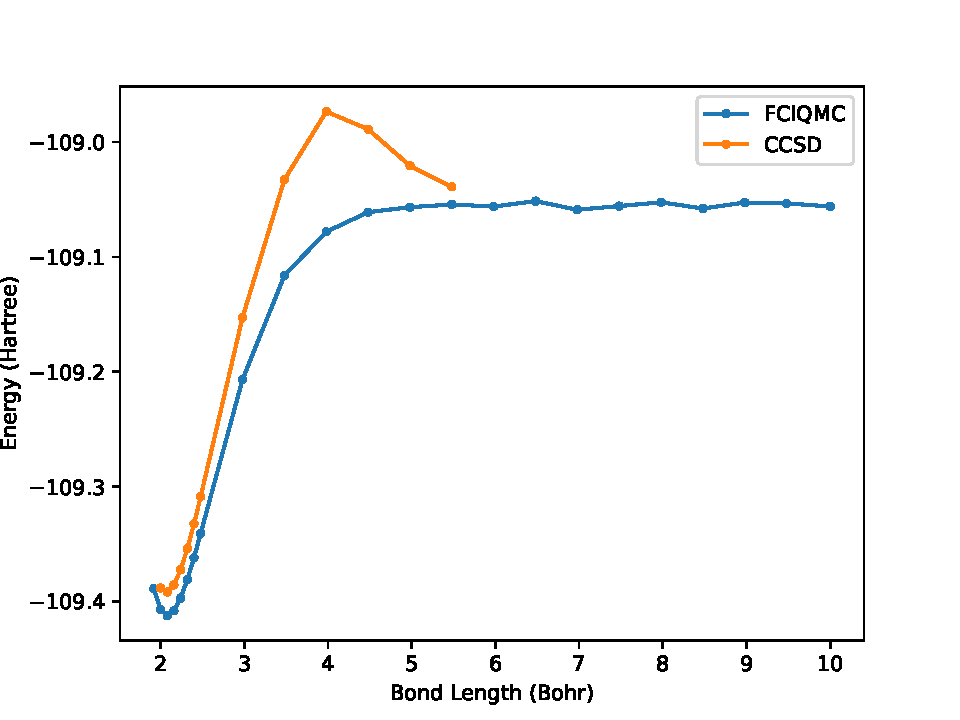
\includegraphics[width=0.8\textwidth]{figures/binding/N2_avtz_nontc}
    \caption{The binding curve for N$_2$ with the \avdz basis set. CCSD starts to decrease near 4 Bohr, which is nonphysical, whereas FCIQMC provides a more accurate curve. FCIQMC was done with 30 million walkers and HF-projected energy. The nonsmooth region in the dissociated region is due to stochastic error, and could be resolved with more walkers and a better trial wave function. CCSD did not converge at bond lengths larger than those shown.}
    \label{fig:ccsd-vs-fciqmc-n2}
\end{figure}

To see how well TC fares against such problems, consider the methodology outlined in chapter \ref{chap:opt}. We again use the same Jastrow factor as in equation \ref{eq:jastrow},
\begin{equation}
    \label{eq:jastrow-again}
    J = \sum_{i<j}^Nv(r_{ij}) + \sum_i^N\sum_I^{N_A}\chi(r_{iI}) + \sum_{i<j}^N\sum_I^{N_A}f(r_{ij}, r_{iI}, r_{jI}),
\end{equation}
with
\begin{equation}
    \label{eq:dtn-jastrow-ee-2}
    v(r_{ij})    = t(r_{ij},L_v)
                    \sum_{k} a_k r_{ij}^k ,
\end{equation}
\begin{equation}
    \label{eq:dtn-jastrow-en-2}
    \chi(r_{iI}) = t(r_{iI},L_\chi)
    \sum_{k} b_k r_{iI}^k ,
\end{equation}
\begin{equation}
    \label{eq:dtn-jastrow-een-2}
    f(r_{ij}, r_{i}, r_{j}) = t(r_{iI},L_f) t(r_{jI},L_f)
    \sum_{k,l,m} c_{klm}
    r_{ij}^k r_{iI}^l r_{jI}^m ,
\end{equation}
and the same cutoff functions $t(r,L) = (1-r/L)^3
\Theta(r-L)$. We also use the same objective function,
\begin{equation}
    \label{eq:varref-hf}
    \sigma_\mathrm{ref}^2 = \sum_{I\neq \mathrm{HF}}\bra{D_I}\htc\ket{D_\mathrm{HF}},
\end{equation}
Using this workflow with the xTC approximation, we calculate points along the binding curve of N$_2$, and find a non-physical ``dip'', as shown in figure \ref{fig:binding-dip}, similar to what CCSD shows exhibits in figure \ref{fig:ccsd-vs-fciqmc-n2}, albeit much more subtle.

\begin{figure}[htbp]
    \centering
    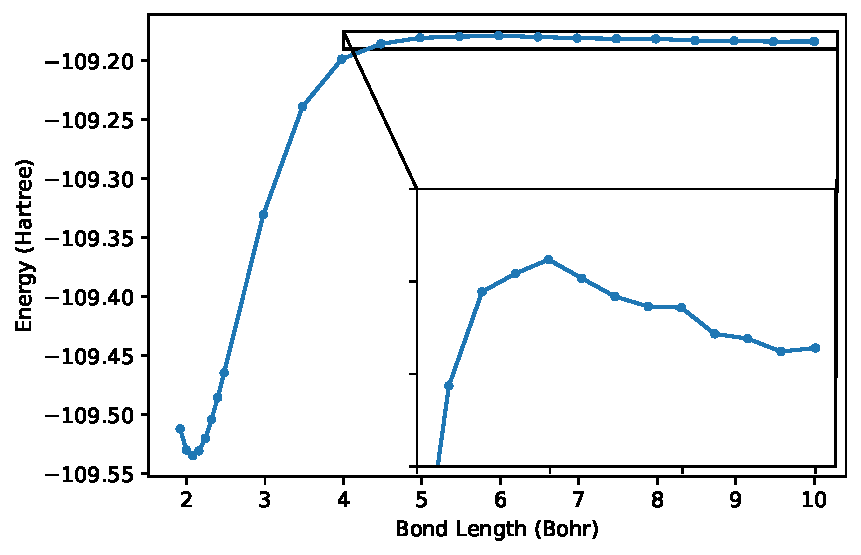
\includegraphics[width=0.8\textwidth]{figures/binding/inset_nontcfciqmc}
    \caption{The xTC-FCIQMC binding curve for N$_2$ with the \avtz basis set. While much smaller than that in figure \ref{fig:ccsd-vs-fciqmc-n2}, a non-physical dip is still present. This is apparent when zooming in on the curve, as shown in the inset.}
    \label{fig:binding-dip}
\end{figure}

This result has been verified for a few points with full TC, which rules out xTC as the issue. Since the post-Hartree-Fock treatment was essentially at the FCI level, this implies that there is something wrong with the calculation of the Jastrow factors themselves. That is, our Hamiltonian is already ``corrupted'' before we even start the post-HF calculation.



\todo{problem description, including the ``dip''}

\todo{mention where things need to change: objective function and sampling, Jastrow ansatz, 1RDM for xTC}

\section{Size Consistency}

\subsection{Jastrow Factor Forms}

\subsection{Multireference Ansatzes}

\todo{Present: "circular" approach, CASCI, CASSCF}

% \todo{present the bad data :( -- mention might hint at needing the core (I think Andreea's paper corroborated this)}

\section{Transcorrelated Trial Wavefunction}

\section{Results}

\subsection{Binding Curves}
\todo{mention that we fix the binding curves}
\todo{also include a table about just ``how size-consistent'' the results actually are.}

\subsection{Excitation Energies}
\todo{mention can target the exact state(s) in question}

% \begin{table}[htbp]
%     \centering
%     \begin{tabular}{c|c|c|c}
%         Molecule & State & \avdz & \avtz & \avqz \\
%         \hline
%         N$_2$ & $^1\Sigma_g^+$ & & & \\
%     \end{tabular}
%     \caption{\todo{excitation energies for a couple of molecules, in mHa}}
%     \label{tbl:excitation-energies}
% \end{table}

\section{Conclusion and Outlook}
\todo{make sure to mention the cutoff analysis and constructing Jastrow factors from atomic Jastrow factors. Mention ECPs, since it's already been submitted...}
\todo{TC-CAS...}
\todo{self-consistent TC (i.e. feed back into itself)}
